%!TEX TS-program = xelatex

\documentclass[a4paper,12pt]{article}

%%% Работа с русским языком
\usepackage[english,russian]{babel}   %% загружает пакет многоязыковой вёрстки
\usepackage{fontspec}      %% подготавливает загрузку шрифтов Open Type, True Type и др.
\defaultfontfeatures{Ligatures={TeX},Renderer=Basic}  %% свойства шрифтов по умолчанию
\setmainfont[Ligatures={TeX,Historic}]{Calibri} %% задаёт основной шрифт документа
\setsansfont{Comic Sans MS}                    %% задаёт шрифт без засечек
\setmonofont{Courier New}
\usepackage{indentfirst}
\frenchspacing

\renewcommand{\epsilon}{\ensuremath{\varepsilon}}
\renewcommand{\phi}{\ensuremath{\varphi}}
\renewcommand{\kappa}{\ensuremath{\varkappa}}
\renewcommand{\le}{\ensuremath{\leqslant}}
\renewcommand{\leq}{\ensuremath{\leqslant}}
\renewcommand{\ge}{\ensuremath{\geqslant}}
\renewcommand{\geq}{\ensuremath{\geqslant}}
\renewcommand{\emptyset}{\varnothing}

%%% Дополнительная работа с математикой
\usepackage{amsmath,amsfonts,amssymb,amsthm,mathtools} % AMS
\usepackage{icomma} % "Умная" запятая: $0,2$ --- число, $0, 2$ --- перечисление

%% Номера формул
%\mathtoolsset{showonlyrefs=true} % Показывать номера только у тех формул, на которые есть \eqref{} в тексте.
%\usepackage{leqno} % Нумерация формул слева	

%% Перенос знаков в формулах (по Львовскому)
\newcommand*{\hm}[1]{#1\nobreak\discretionary{}
	{\hbox{$\mathsurround=0pt #1$}}{}}

%%% Работа с картинками
\usepackage{graphicx}  % Для вставки рисунков
\graphicspath{{images/}}  % папки с картинками
\setlength\fboxsep{3pt} % Отступ рамки \fbox{} от рисунка
\setlength\fboxrule{1pt} % Толщина линий рамки \fbox{}
\usepackage{wrapfig} % Обтекание рисунков текстом

%%% Работа с таблицами
\usepackage{array,tabularx,tabulary,booktabs} % Дополнительная работа с таблицами
\usepackage{longtable}  % Длинные таблицы
\usepackage{multirow} % Слияние строк в таблице
\usepackage{float}% http://ctan.org/pkg/float

%%% Программирование
\usepackage{etoolbox} % логические операторы


%%% Страница
\usepackage{extsizes} % Возможность сделать 14-й шрифт
\usepackage{geometry} % Простой способ задавать поля
\geometry{top=20mm}
\geometry{bottom=20mm}
\geometry{left=30mm}
\geometry{right=15mm}
%
%\usepackage{fancyhdr} % Колонтитулы
% 	\pagestyle{fancy}
%\renewcommand{\headrulewidth}{0pt}  % Толщина линейки, отчеркивающей верхний колонтитул
% 	\lfoot{Нижний левый}
% 	\rfoot{Нижний правый}
% 	\rhead{Верхний правый}
% 	\chead{Верхний в центре}
% 	\lhead{Верхний левый}
%	\cfoot{Нижний в центре} % По умолчанию здесь номер страницы

\usepackage{setspace} % Интерлиньяж
\onehalfspacing % Интерлиньяж 1.5
%\doublespacing % Интерлиньяж 2
%\singlespacing % Интерлиньяж 1

\usepackage{lastpage} % Узнать, сколько всего страниц в документе.

\usepackage{soul} % Модификаторы начертания

\usepackage{hyperref}
\usepackage[usenames,dvipsnames,svgnames,table,rgb]{xcolor}
\hypersetup{				% Гиперссылки
	unicode=true,           % русские буквы в раздела PDF
	pdftitle={Отчет о прохождении практики},   % Заголовок
	pdfauthor={Самоделкина М.В.},      % Автор
	pdfsubject={Отчет о прохождении практики},      % Тема
	pdfcreator={Самоделкина М.В.}, % Создатель
	pdfproducer={Самоделкина М.В.}, % Производитель
	pdfkeywords={keyword1} {key2} {key3}, % Ключевые слова
	colorlinks=true,       	% false: ссылки в рамках; true: цветные ссылки
	linkcolor=blue,          % внутренние ссылки
	citecolor=black,        % на библиографию
	filecolor=magenta,      % на файлы
	urlcolor=blue           % на URL
}
\makeatletter 
\def\@biblabel#1{#1. } 
\makeatother
\usepackage{cite} % Работа с библиографией
%\usepackage[superscript]{cite} % Ссылки в верхних индексах
%\usepackage[nocompress]{cite} % 
\usepackage{csquotes} % Еще инструменты для ссылок

\usepackage{multicol} % Несколько колонок

\usepackage{tikz} % Работа с графикой
\usepackage{pgfplots}
\usepackage{pgfplotstable}

% ГОСТ заголовки
\usepackage[font=small]{caption}
%\captionsetup[table]{justification=centering, labelsep = newline} % Таблицы по правобу краю
%\captionsetup[figure]{justification=centering} % Картинки по центру
\usepackage{ dsfont }

\newcommand{\tablecaption}[1]{\addtocounter{table}{1}\small \begin{flushright}\tablename \ \thetable\end{flushright}%	
\begin{center}#1\end{center}}

\newcommand{\imref}[1]{рис.~\ref{#1}}

\usepackage{multirow}
\usepackage{spreadtab}
\newcolumntype{K}[1]{@{}>{\centering\arraybackslash}p{#1cm}@{}}


\usepackage{xparse}
\usepackage{fancyvrb}

\RecustomVerbatimCommand{\VerbatimInput}{VerbatimInput}
{
	fontsize=\footnotesize    
}

\newcolumntype{?}[1]{!{\vrule width #1}}

\usepackage{tocloft}
\renewcommand{\cftsecleader}{\cftdotfill{\cftdotsep}}

\usepackage{pdfpages}

\usepackage{longtable}
\begin{document} % конец преамбулы, начало документа
\begin{titlepage}
	\begin{center}
		ПРАВИТЕЛЬСТВО РОССИЙСКОЙ ФЕДЕРАЦИИ \\
 		ФЕДЕРАЛЬНОЕ  ГОСУДАРСТВЕННОЕ АВТОНОМНОЕ \\
		ОБРАЗОВАТЕЛЬНОЕ УЧРЕЖДЕНИЕ ВЫСШЕГО ОБРАЗОВАНИЯ\\
		«НАЦИОНАЛЬНЫЙ ИССЛЕДОВАТЕЛЬСКИЙ УНИВЕРСИТЕТ\\
		«ВЫСШАЯ ШКОЛА ЭКОНОМИКИ»
	\end{center}
	
	\begin{center}
		\textbf{Московский институт электроники и математики}
		
		\textbf{Им. А.Н.Тихонова НИУ ВШЭ}
		
		\vspace{2ex}
		
		\textbf{Направление 01.03.04. Прикладная математика \\
			Бакалаврская программа <<Прикладная математика>>}
	\end{center}
	\vspace{1ex}	
	
	\vspace{1ex}
	\begin{center}
		\textbf{Отчет по самостоятельной работе \\
			по дисциплине <<Методы анализа стохастических взаимосвязей>>\\
			часть 1
	}
	\end{center}	

	\vspace{2ex}
	\vfill
	
	\vspace{2ex}
	
	\begin{flushright}
		\textbf{Бригада №7:}
		
		\vspace{2ex}
		
		Ремизова Анна Петровна, 4 курс, БПМ174
		
		Самоделкина Мария Владимировна, 4 курс, БПМ174

	\end{flushright}

	\vspace{5ex}
	\begin{center}
		Москва \the\year \, г.
	\end{center}
	
\end{titlepage}
\addtocounter{page}{1}
%\title{Отчет о прохождении производственной практики}
%\date{}
%\maketitle
%\includepdf{data/title2.pdf}
\tableofcontents
\pagebreak

\section{Общая постановка задачи}
\subsection{Формулировка прикладной проблемы}
В настоящее время в связи со сложной эпидемиологической обстановкой в мире очень актуально медицинское страхование. В частности США является лидером по заболеваемости от COVID-19 по информации с сайта Всемирной Организации Здравоохранения. Как известно, медицинское обслуживание в этой стране имеет страховой характер. По данным сайта переписи населения США 91,5\% населения США имеет медицинскую страховку. Следовательно, большая часть людей заинтересованы в ее приобретении. При этом размер страхового взноса зависит от параметров потребителя, и чаще всего вычисляется индивидуально. В связи с этим для актуария встает проблема определения размера страхового взноса для разных категорий населения.

В данной работе рассматривается задача определения размера минимального индивидуального взноса для конкретной категории населения, а именно
для некурящих женщин в возрасте 19–44 лет с индексом массы тела в диапазоне от 18,5 до 25. Наш выбор обосновывается тем, что по статистике женщины на 32\% чаще мужчин берут страховку, а остальные параметры соответствуют среднестатистическому здоровому человеку.
%Определение размера индивидуальных взносов медицинского страхования по информации о человеке: полу, возрасту, индексу массы тела, количеству детей, наличию вредных привычек и региону.

\subsection{Потенциальные потребители решения. Задачи, которые они смогут решать,	используя полученные результаты}
Полученные решения будут применяться медицинскими страховыми компаниями в США. Набор данных соответствует северным районам США - в них находятся мегалополисы с большой численностью населения.

Используя полученные результаты, потребители смогут оценивать размер индивидуальных взносов, основываясь на индивидуальных характеристиках человека.

\subsection{Основные гипотезы, которые планируется проверить в рамках решения задачи}
В таблице \ref{tab:table1} представлены индивидуальные характеристики человека, используемые для анализа медицинских взносов. 

\begin{table}[H]
\begin{center}
	\begin{tabular}{ | l | p{4cm} | p{2.6cm} | p{4.2cm} | p{3.7cm} |}
		\hline
		№ & Характеристика объекта & Название переменной & Шкала измерения & Роль переменной \\ \hline
		1 & Возраст & age & Относительная & Независимая \\ \hline
		2 & Пол & sex & Номинальная (дихотомическая) & Независимая \\ \hline
		3 & Индекс массы тела & bmi & Относительная & Независимая \\ \hline
		4 & Число детей & children & Относительная & Независимая \\ \hline
		5 & Наличие вредных привычек (курение) & smoker & Номинальная (дихотомическая) & Независимая \\ \hline
		6 & Индивидуальные взносы & charges & Относительная & Зависимая \\ \hline
	\end{tabular}
\end{center}
\caption{Описание факторов, учтенных в анализе.}
\label{tab:table1}
\end{table}
Сформулируем гипотезы о статистической взаимосвязи зависимых и независимых переменных:
\begin{enumerate}
	\item У людей с вредными привычками размер страховых взносов больше, чем у людей без вредных привычек. Это обосновывается тем, что у курящих людей вероятность заболеваний дыхательных путей выше, что приводит к страховым случаям.
	%\item Индекс массы тела человека до некоторого возраста растет, а затем уменьшается.
	
	\item С ростом индекса массы тела, после некоторого значения, сила его влияния увеличивается. Это связывается с тем, что люди с чрезмерно высоким весом чаще подвержены заболеваниям сердечно-сосудистой системы. 
	%\item Цена медицинской страховки уменьшается с увеличением индекса массы тела до 18.5, затем размер взносов практически не меняется в зависимости от индекса массы тела в промежутке от 18,5 до 25, а затем с увеличением индекса снова растет. Это связывается с тем, что люди с чрезмерно низким и высоким весом чаще подвержены заболеваниям сердечно-сосудистой системы. 
	
	\item С возрастом размер медицинских страховых взносов растет. При этом скорость роста взносов у мужчин с возрастом выше, чем у женщин. Эта гипотеза подкреплена тем, что по статистике у пожилых людей больше хронических заболеваний и выше вероятность их обострения. При этом средняя продолжительность жизни женщин выше, чем у мужчин, что также отражается на частоте страховых случаев.
\end{enumerate}

\subsection{Основные источники данных}
Основные источники данных, использованные в работе.
\begin{enumerate}
	\item Данные были взяты из \href{https://github.com/stedy/Machine-Learning-with-R-datasets/blob/master/insurance.csv}{репозитория в GitHub};
	\item Информация по заболеваемости COVID-19 доступна на \href{https://covid19.who.int/}{сайте Всемирной Организации Здравоохранения};
	\item Интервал нормы индекса массы тела здорового человека нашли на  \href{https://www.cdc.gov/healthyweight/assessing/bmi/adult_bmi/index.html}{сайте департамента здоровья США};
	\item Статистика по процентам застрахованного населения США взята с \href{https://www.census.gov/library/publications/2019/demo/p60-267.html#:~:text=The%20percentage%20of%20people%20with,in%202017%20(92.1%20percent).}{официального сайта перепеси населения США}.
	\item Различия по частоте страхования между мужчинами и женщинами и выделение возрастной группы женщин взяты из статьи Cylus J. et al. Pronounced gender and age differences are evident in personal health care spending per person //Health Affairs. – 2011. – Т. 30. – №. 1. – С. 153-160.
	
\end{enumerate}

\section{Предварительный анализ собранных данных}
\subsection{Анализ особенностей данных}
\subsubsection{Анализ количественных переменных}

\begin{figure}[h]
	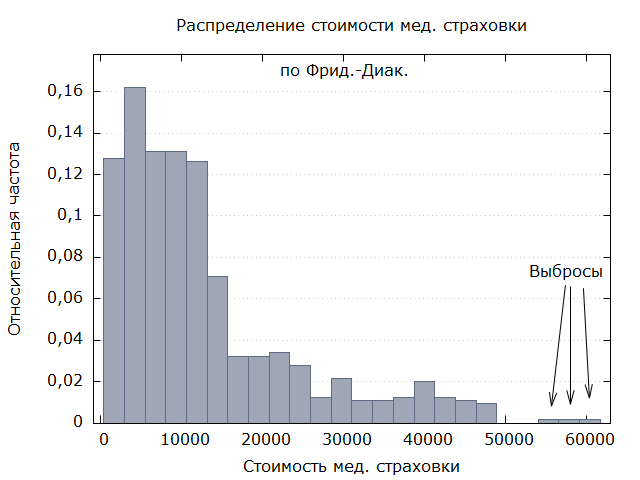
\includegraphics[width=0.6\textwidth]{../[graphics]/charges.png}
	\centering
	\caption{Стоимость страховки}
	\label{fig:charges}
\end{figure}

На основании анализа гистограммы рис.\ref{fig:charges} и описательных статистик табл.\ref{tab:table2} следует сделать вывод о том, что распределение целевой переменной ассимметрично вправо. Это объясняется тем, что основная часть клиентов платит относительно средние суммы. Но есть и другая группа людей с повышенными медицинскими рисками, их не так много, но цена страховки для них выше. Хвост распределния очень длинный, это объясняется тем, что наблюдается большая вариативность в стоимости страховки. Есть выбросы с заметно большей стоимостью медицинской страховки, их доля очень мала. Полимодальности нет, естественной группировки нет.

\begin{figure}[h]
	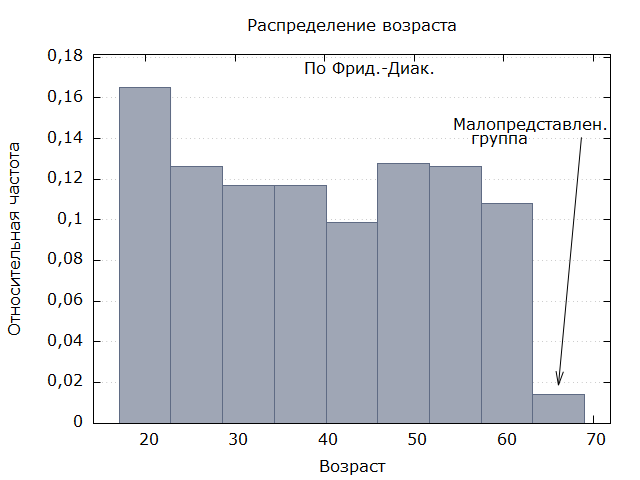
\includegraphics[width=0.6\textwidth]{../[graphics]/age.png}
	\centering
	\caption{Возраст}
	\label{fig:age}
\end{figure}

Распределение возраста (рис. \ref{fig:age}, табл.\ref{tab:table2}) ассимметрично вправо. По виду гистограммы можно говорить о наличии двух кластеров: молодых людей в возрасте от 18 до 23 лет и людей, старше 23 лет. Респонденты в возрасте 18-23 лет резко выделяются, они широкопредставлены в выборке. Это отражает особенность системы страхования: у молодых людей заканчивается детская страховка и они массово оформляют взрослый вариант впервые. Остальные группы возрастов равнопредставленны. Это отражает свойство генеральной свокупности, а именно, что представители каждого возраста имеют одинаковый процент застрахованных, который практически неизменен, люди продлевают страховку из года в год. Группа людей в возрасте от 63 до 69 лет малопредставленна, что частично отражает свойство генеральной совокупности, так как часть людей не доживает до такого возраста. Также малопредставленность может быть обусловлена тем, что люди пожилого возраста не берут страховку, поскольку она для них дорогая и они не могут себе ее позволить. В свою очередь страховщики неохотно оформляют или оформляют по завышенной цене медицинскую страховку из-за больших рисков потерять средства. Полимодальности нет.

\begin{figure}[h]
	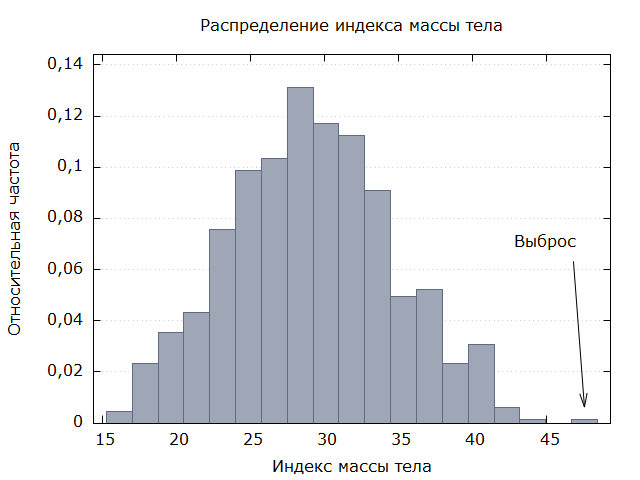
\includegraphics[width=0.6\textwidth]{../[graphics]/bmi.png}
	\centering
	\caption{Индекс массы тела}
	\label{fig:bmi}
\end{figure}

На основании анализа гистограммы рис.\ref{fig:charges} и описательных статистик табл.\ref{tab:table2} следует сделать вывод о том, что распределение индекса массы тела близко к нормальному, с незначительной правосторонней асимметрией. Действительно, согласно последним исследованиям, среди американцев преобладают люди с избыточной массой тела. Ниже в табл.\ref{tab:bmi} представлена итерпретация ИМТ в соответсвии с рекомендациями ВОЗ.

\begin{table}[H]
	\begin{center}
		\begin{tabular}{ | l | l |}
			\hline
			ИМТ & Интерпретация \\ \hline
			Менее 18,5 & Дефицит массы тела \\ \hline
			18,5 - 24,9 & Норма \\ \hline
			25,0 - 29,9 & Избыточная масса тела \\ \hline
			Более 30,0 & Ожирение \\ \hline
		\end{tabular}
	\end{center}
	\caption{Интерпретация ИМТ в соответствии с рекомендациями ВОЗ.}
	\label{tab:bmi}
\end{table}

Медиана и среднее нахордятся в диапазоне избыточной массы тела, что также подтвержает свойства генеральной совокупности.

Кроме того, хорошо заметен выброс с аномально большой массой тела, что также согласуется с действительностью.

\begin{table}[H]
\begin{center}
	\begin{tabular}{|lr@{,}lr@{,}lr@{,}lr@{,}l|}
		\hline
		Переменная & \multicolumn{2}{c}{Среднее}
		& \multicolumn{2}{c}{Медиана}
		& \multicolumn{2}{c}{Минимум}
		& \multicolumn{2}{c|}{Максимум} \\[1ex]
		\hline
		age & 39&233 & 39&000 & 18&000 & 64&000\\
		bmi & 29&187 & 28&880 & 15&960 & 48&070\\
		children & 1&0971 & 1&0000 & 0&00000 & 5&0000\\
		charges & 12911& & 9644&3 & 1621&3 & 60021&\\[10pt]
		
		\hline
		Переменная &  \multicolumn{2}{c}{Ст.\ Откл.}
		& \multicolumn{2}{c}{Вариация}
		& \multicolumn{2}{c}{Асимметрия}
		& \multicolumn{2}{c|}{Эксцесс} \\[1ex]
		\hline
		age & 14&050 & 0&35811 & 0&051080 & $-$1&2547\\
		bmi & 5&5467 & 0&19004 & 0&15599 & $-$0&25062\\
		children & 1&1856 & 1&0807 & 0&79614 & $-$0&30309\\
		charges & 11167& & 0&86488 & 1&5758 & 2&1084\\[10pt]
		
		\hline
		Переменная &  \multicolumn{2}{c}{5\% проц.}
		& \multicolumn{2}{c}{95\% проц.}
		& \multicolumn{2}{c}{IQ Range}
		& \multicolumn{2}{c|}{Пропущенные наблюдения} \\[1ex]
		\hline
		age & 18&500 & 61&500 & 25&000 & \multicolumn{2}{c|}{0}\\
		bmi & 19&998 & 39&045 & 7&5525 & \multicolumn{2}{c|}{0}\\
		children & 0&00000 & 3&0000 & 2&0000 & \multicolumn{2}{c|}{0}\\
		charges & 2135&9 & 39661& & 11043& & \multicolumn{2}{c|}{0}\\
		\hline
	\end{tabular}
\end{center}
\caption{Описательные статистики количественных переменных.}
\label{tab:table2}
\end{table}

\subsubsection{Анализ качественных переменных}

\begin{figure}[H]
	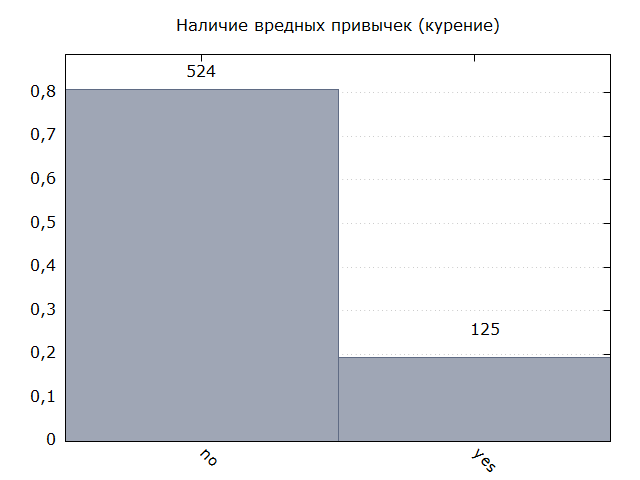
\includegraphics[width=0.6\textwidth]{../[graphics]/smoker.png}
	\centering
	\caption{Наличие вредных привычек}
	\label{fig:smoker}
\end{figure}

По признаку наличия вредных привычек выборка не является сбалансированной (рис. \ref{fig:smoker}), что есть естественное свойство генеральной совокупности: в действительности некурящих людей больше, чем курящих. Агрегацию уровней проводить не требуется, группы курящих и некурящих людей не являются малопредставленными.

\begin{figure}[H]
	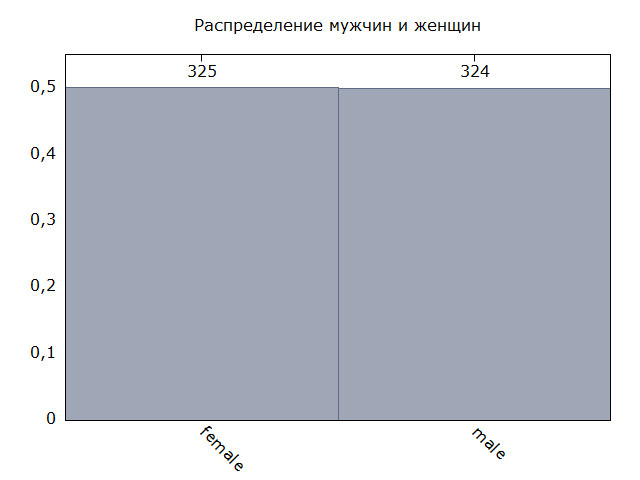
\includegraphics[width=0.6\textwidth]{../[graphics]/sex.png}
	\centering
	\caption{Пол}
	\label{fig:sex}
\end{figure}

Выборка сбалансирована по полу - представлено равное количество мужчин и женщин. Это отражает репрезентативность выборки.

\subsection{Анализ статистической связи}

\subsubsection{Графический анализ пары «числовая зависимая переменная – качественная независимая переменная»}

\subsubsection{Графический анализ пары «числовая зависимая переменная – числовая независимая переменная»}

\begin{figure}[h]
	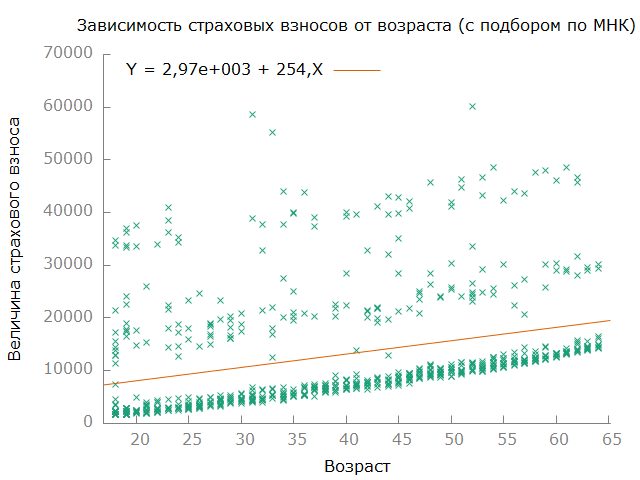
\includegraphics[width=0.6\textwidth]{../[graphics]/age-price.png}
	\centering
	\caption{Зависимость страховых взносов от возраста}
	\label{fig:age-price}
\end{figure}

Анализируя график на рисунке \ref{fig:age-price}, можно выделить 3 группы людей: здоровые люди (некурящие, с небольшим индексом массы тела), группа с отклонениями в здоровье и группа людей со значительными отклонениями в здоровье (курящие и с ожирением). 

Для каждой такой группы людей видна явная линейная зависимость цены страховки от возраста. Причем коэффициент роста цены на страховку с возрастом визуально одинаковый для всех установленных групп людей. Множитель при возрасте в рассматриваемой линейной зависимости можно интерпретировать как надбавку в стоимости страховки за возраст. При этом цены на страховку в каждой группе людей сильно отличаются значением свободного коэффициента. Для здоровых людей этот коэффициент низкий, поскольку риски заболевания у них небольшие. Для остальных групп этот коэффициент будет выше, поскольку вероятность страхового случая для людей с отклонениями в здоровье значительно выше. 

Также стоит отметить, что разброс значений в стоимости страховки у первой группы людей значительно меньше, чем у других групп. Это объясняется тем, что в первой группе находятся здоровые люди: двум здоровым людям одного возраста положена страховка одинаковой стоимости, поскольку они по состоянию здоровья практически не отличаются. В это же время люди с отклонениями в здоровье могут иметь разные осложнения и разные степени заболевания, что сказывается и на стоимости.

На графике можно наблюдать выбросы, которые не описываются ни одной из обозначенных линейных зависимостей. При этом нет выбросов ниже линейной зависимости для первой группы людей. Действительно, абсолютно здоровому человеку страховщик не будет уменьшать цену, цена может только увеличиваться, если у человека есть какие-либо заболевания. 

\subsubsection{Анализ наличия корреляции между независимыми переменными}

\subsubsection{Предварительная проверка гипотез}

\section{Спецификация, оценивание и оптимизация модели}

\subsection{Спецификация моделей для проверки гипотез и решения поставленной задачи}

\subsection{Оценивание базовой модели и результаты проверки гипотез}

\subsection{Анализ наличия выбросов}

\subsection{Анализ наличия гетероскедастичности}

\subsection{Оптимизация модели}

\subsection{Проверка прогностических свойств модели}

\section{Выводы и рекомендации}

\end{document} % конец документа